% Entity-relationship diagram
\documentclass{article}
\usepackage{ngerman}
\usepackage{tikz}
\usetikzlibrary{er,positioning}
\begin{document}
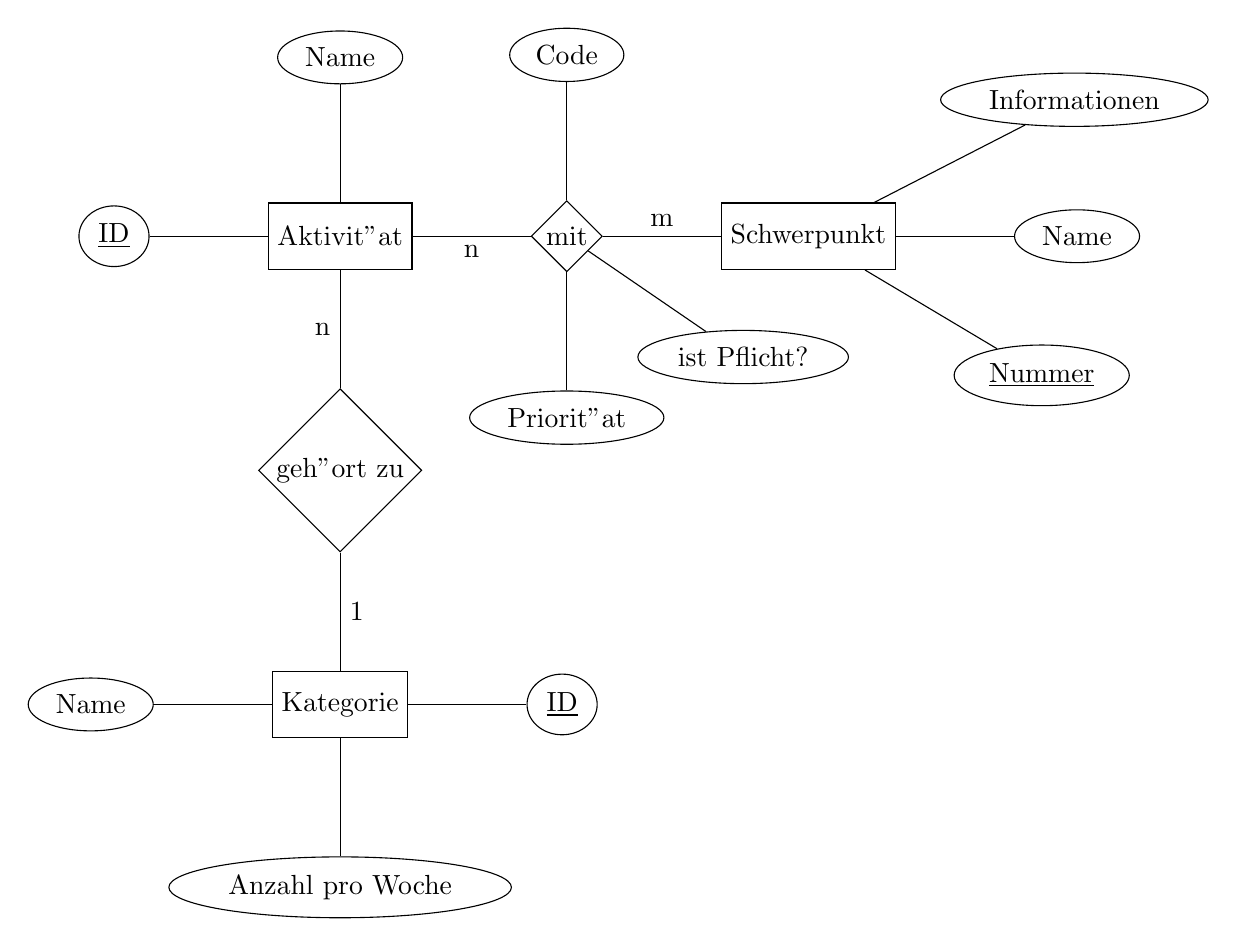
\begin{tikzpicture}[auto,node distance=1.5cm]
  \node[entity] (activity) {Aktivit"at};
    \node[attribute] (activity_name) [above =of activity] {Name} edge (activity);
  	\node[attribute] (activity_id) [left  =of activity] {\underline{ID}} edge (activity);

  \node[relationship] (mit) [right = of activity] {mit};
  	\node[attribute] (code) [above =of mit] {Code} edge (mit);
  	\node[attribute] (priority) [below  =of mit] {Priorit"at} edge (mit);
  	\node[attribute] (pflicht) [below right=of mit] {ist Pflicht?} edge (mit);

  \node[entity] (schwerpunkt) [right = of mit]	{Schwerpunkt};
  	\node[attribute] (information) [above right =of schwerpunkt] {Informationen} edge (schwerpunkt);
  	\node[attribute] (schwerpunkt_name) [right =of schwerpunkt] {Name} edge (schwerpunkt);
  	\node[attribute] (number) [below right =of schwerpunkt] {\underline{Nummer}} edge (schwerpunkt);

  \path (mit) edge node {n} (activity) edge node {m} (schwerpunkt);
    
  \node[relationship] (belongs_to) [below = of activity] {geh"ort zu};

  \node[entity] (category) [below = of belongs_to]	{Kategorie};
  	\node[attribute] (per_week) [below =of category] {Anzahl pro Woche} edge (category);
  	\node[attribute] (category_name) [left =of category] {Name} edge (category);
  	\node[attribute] (category_id) [right=of category] {\underline{ID}} edge (category);

  \path (belongs_to) edge node {n} (activity) edge node {1}	(category);
\end{tikzpicture}
\\ \\
\textbf{Tabellen:}\\
Aktivit"at mit Fremdschl"ussel aus Kategorie, Schwerpunkt, Kategorie, mit
\end{document}